\pdfminorversion=4
\documentclass[aspectratio=169]{beamer}

\mode<presentation>
{
  \usetheme{default}
  \usecolortheme{default}
  \usefonttheme{default}
  \setbeamertemplate{navigation symbols}{}
  \setbeamertemplate{caption}[numbered]
  \setbeamertemplate{footline}[frame number]  % or "page number"
  \setbeamercolor{frametitle}{fg=white}
  \setbeamercolor{footline}{fg=black}
} 

\usepackage[english]{babel}
\usepackage{inputenc}
\usepackage{tikz}
\usepackage{courier}
\usepackage{array}
\usepackage{bold-extra}
\usepackage{minted}
\usepackage[thicklines]{cancel}
\usepackage{fancyvrb}

\xdefinecolor{dianablue}{rgb}{0.18,0.24,0.31}
\xdefinecolor{darkblue}{rgb}{0.1,0.1,0.7}
\xdefinecolor{darkgreen}{rgb}{0,0.5,0}
\xdefinecolor{darkgrey}{rgb}{0.35,0.35,0.35}
\xdefinecolor{darkorange}{rgb}{0.8,0.5,0}
\xdefinecolor{darkred}{rgb}{0.7,0,0}
\definecolor{darkgreen}{rgb}{0,0.6,0}
\definecolor{mauve}{rgb}{0.58,0,0.82}

\title[2024-10-23-chep2024-gil-free-uproot]{GIL-free scaling of Uproot in Python 3.13}
\author{Jim Pivarski}
\institute{Princeton University -- IRIS-HEP}
\date{October 23, 2024}

\usetikzlibrary{shapes.callouts}

\begin{document}

\logo{\pgfputat{\pgfxy(0.11, 7.4)}{\pgfbox[right,base]{\tikz{\filldraw[fill=dianablue, draw=none] (0 cm, 0 cm) rectangle (50 cm, 1 cm);}\mbox{\hspace{-8 cm}
\includegraphics[height=1 cm]{princeton-logo-long.png}\hspace{0.1 cm}\raisebox{0.1 cm}{
\includegraphics[height=0.8 cm]{iris-hep-logo-long.png}}\hspace{0.1 cm}}}}}

\begin{frame}
  \titlepage
\end{frame}

\logo{\pgfputat{\pgfxy(0.11, 7.4)}{\pgfbox[right,base]{\tikz{\filldraw[fill=dianablue, draw=none] (0 cm, 0 cm) rectangle (50 cm, 1 cm);}\mbox{\hspace{-8 cm}
\includegraphics[height=1 cm]{princeton-logo.png}\hspace{0.1 cm}\raisebox{0.1 cm}{
\includegraphics[height=0.8 cm]{iris-hep-logo.png}}\hspace{0.1 cm}}}}}

% Uncomment these lines for an automatically generated outline.
%\begin{frame}{Outline}
%  \tableofcontents
%\end{frame}

% START START START START START START START START START START START START START

\begin{frame}[fragile]{What is Python's Global Interpreter Lock (GIL)?}
\Large
\vspace{0.5 cm}
\begin{onlyenv}<1>
\begin{center}

\includegraphics[height=5 cm]{img/python-gil-meme-1.jpg}
\end{center}
\end{onlyenv}\begin{onlyenv}<2>
\begin{center}

\includegraphics[height=5 cm]{img/python-gil-meme-2.jpg}
\end{center}
\end{onlyenv}\begin{onlyenv}<3>
\begin{center}

\includegraphics[height=5 cm]{img/python-gil-meme-3.png}
\end{center}
\end{onlyenv}\begin{onlyenv}<4>
\hspace{-0.25 cm}\textcolor{darkblue}{In pseudocode:}

\vspace{0.5 cm}
\begin{minted}{c}
 pthread_mutex_lock(&global_interpreter_lock);

 PyEval(python_bytecode_instruction);

 pthread_mutex_unlock(&global_interpreter_lock);
\end{minted}
\end{onlyenv}\begin{onlyenv}<5>
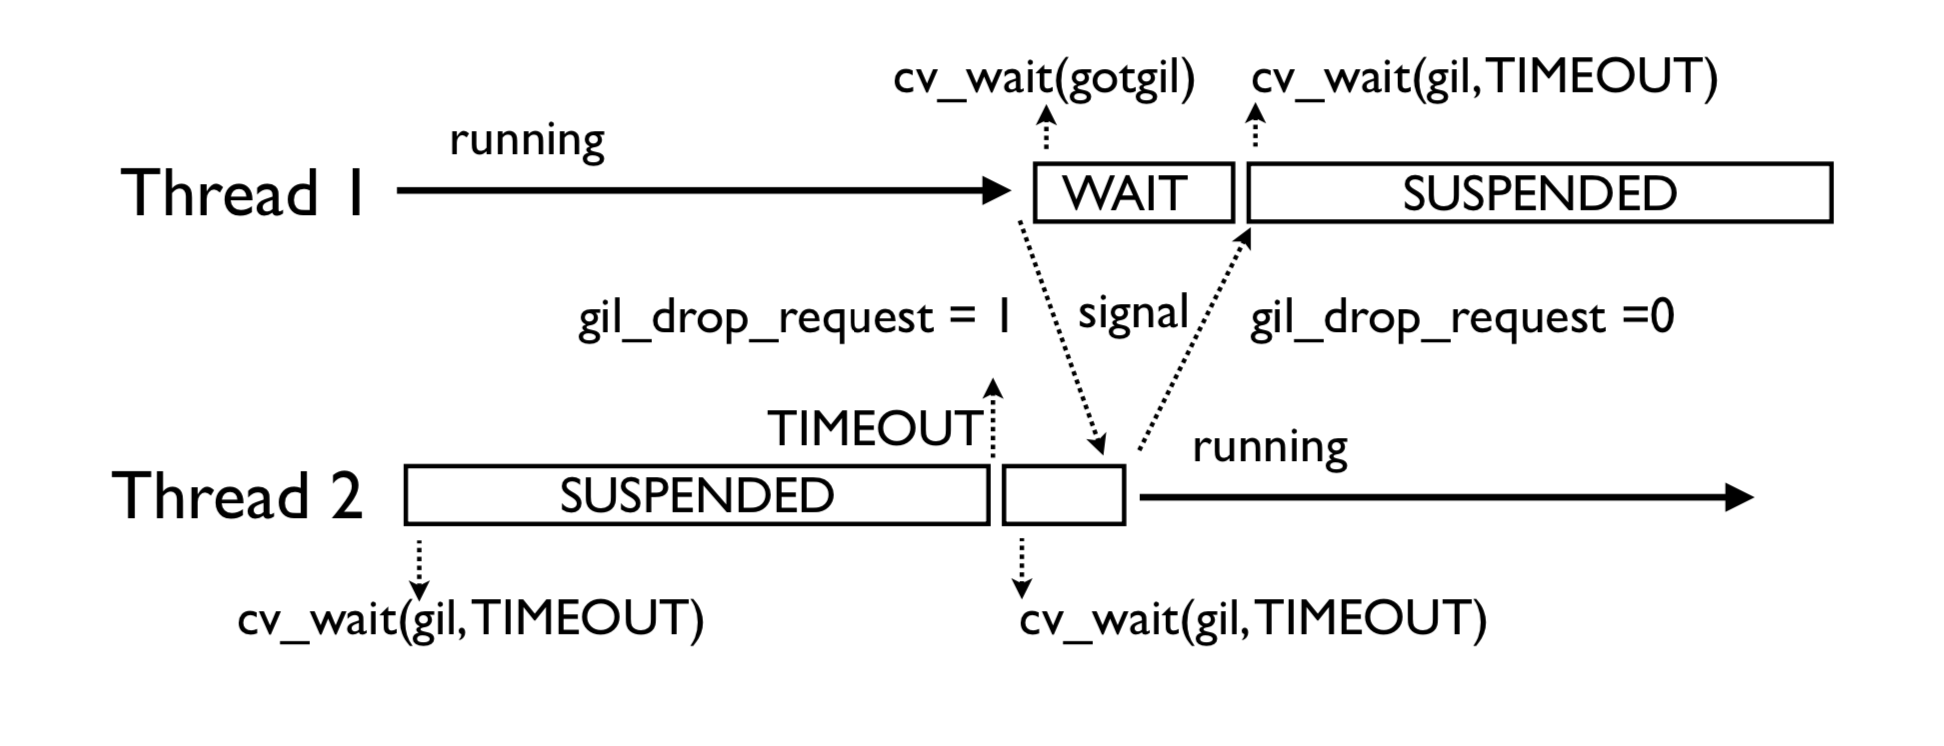
\includegraphics[width=\linewidth]{img/new_gil.png}

\normalsize
\textcolor{blue}{\url{https://github.com/zpoint/CPython-Internals/blob/master/Interpreter/gil/gil.md}}
\end{onlyenv}
\end{frame}

\begin{frame}{\mbox{ }}
\Large
\vspace{0.5 cm}
\begin{center}
Python 3.13.0 was released 16 days ago.

\vspace{1 cm}
\uncover<2>{It adds two new ways to avoid the GIL.}
\end{center}
\end{frame}

\begin{frame}
\vspace{1 cm}
\LARGE
\begin{center}
\textcolor{darkblue}{Method \#1: subinterpreters}
\end{center}
\end{frame}

\begin{frame}{Method \#1: subinterpreters}
\large
\vspace{0.5 cm}
\begin{columns}
\column{1.1\linewidth}
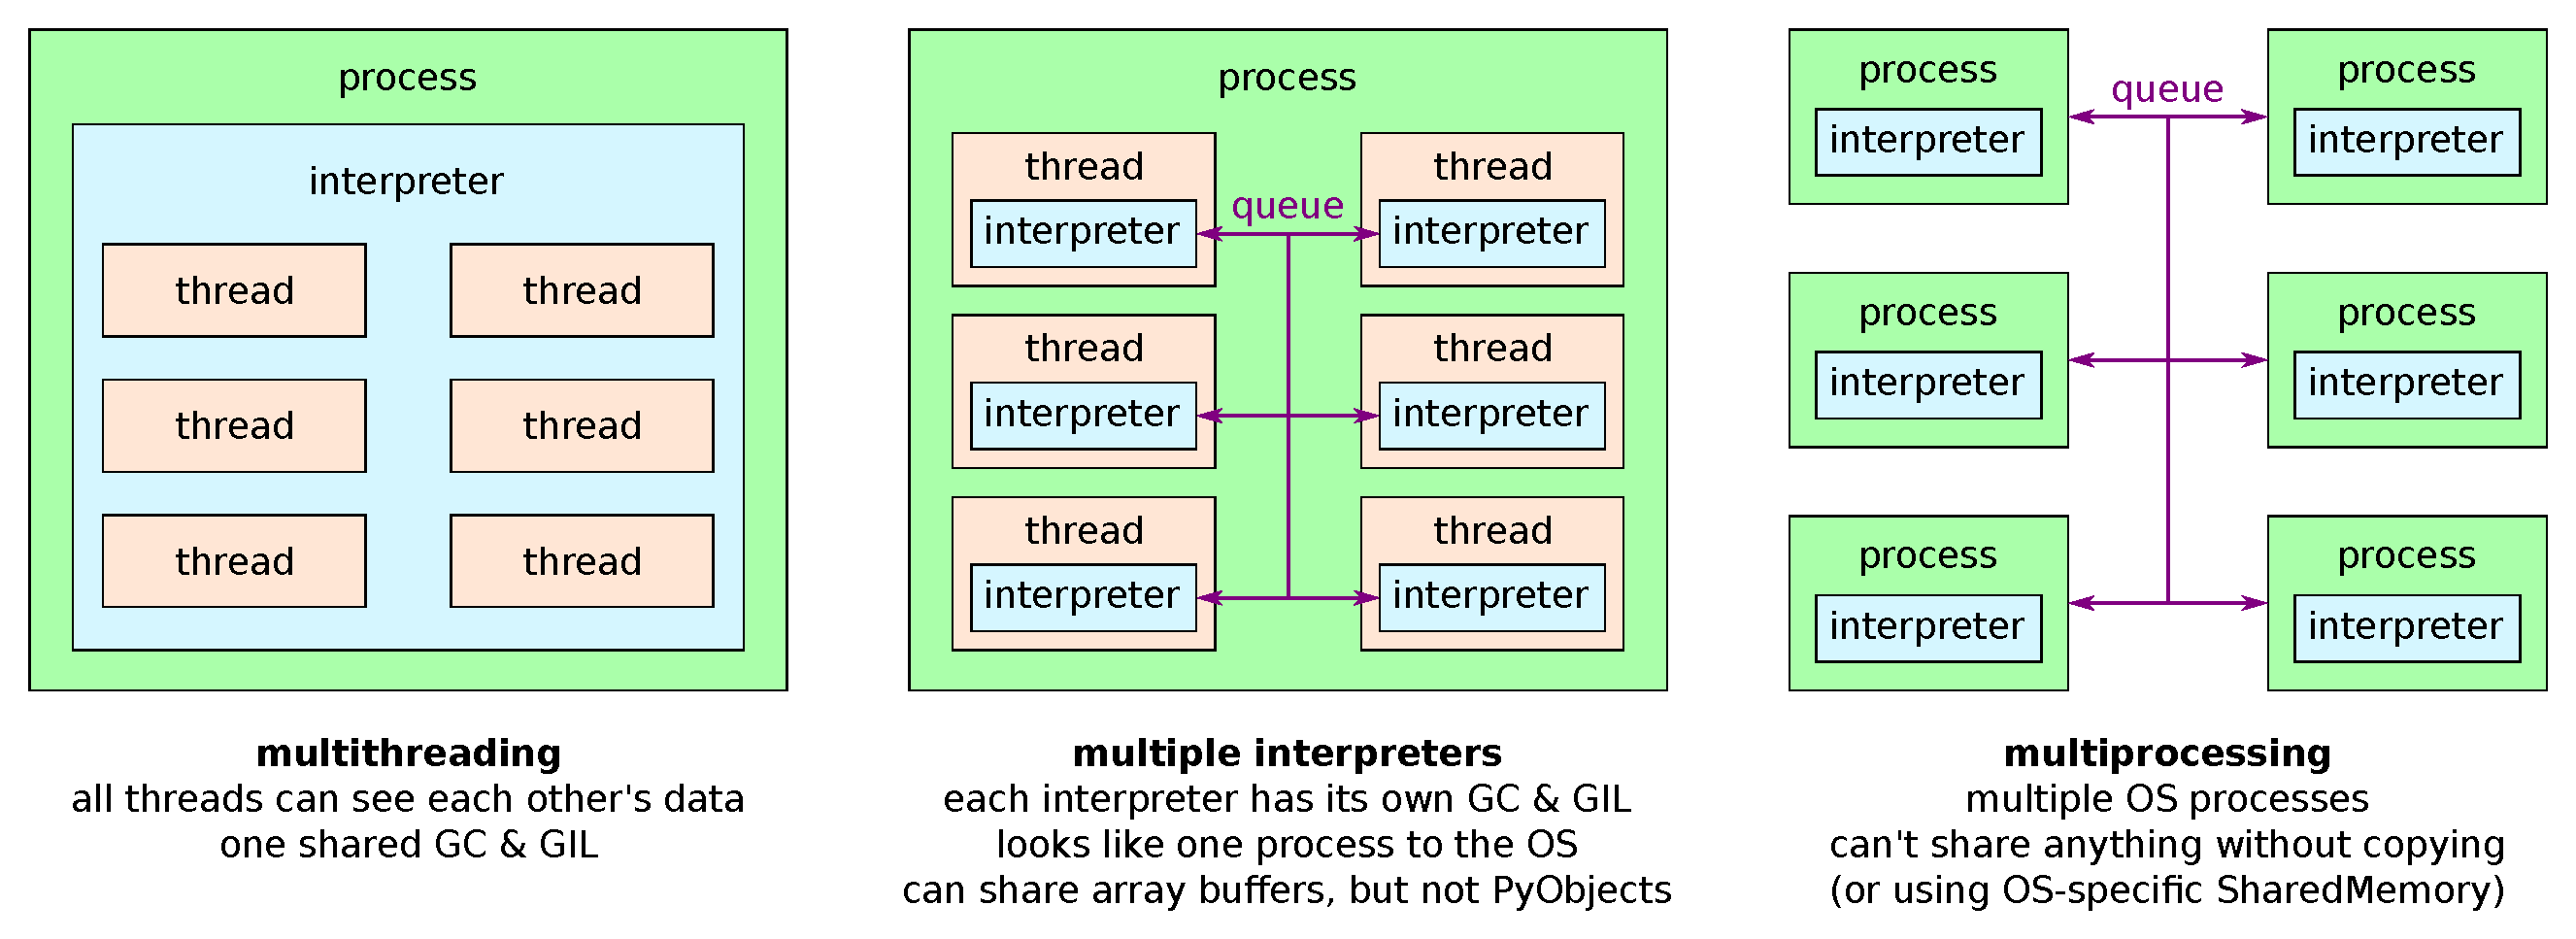
\includegraphics[width=\linewidth]{img/thread-interpreter-process.pdf}
\end{columns}

\vspace{0.5 cm}
\uncover<2>{Pre-3.13 trade-off: shared memory + GIL in {\bf multithreading} or shared-nothing + true parallel-processing in {\bf multiprocessing}. \textcolor{darkblue}{Now we have an in-between option.}}
\end{frame}

\begin{frame}[fragile]{It is now possible, but not easy, to use subinterpreters in Python}
\vspace{0.35 cm}
\scriptsize
\begin{minted}{python}
from test.support import interpreters
from test.support.interpreters import queues

def in_subinterp():
    # Need to re-import; this is in its own little world...
    from test.support.interpreters import queues

    in_queue = Queue(in_id)      # in_id comes from global scope
    out_queue = Queue(out_id)    # out_id comes from global scope

    x = queue.get()
    out_queue.put(x + number)    # number comes from global scope

in_queue = queues.create()
out_queue = queues.create()

subinterp = interpreters.create()
subinterp.prepare_main({"in_id": in_queue.id, "out_id": out_queue.id, "number": 42})
subinterp.call_in_thread(in_subinterp)

in_queue.put(100)
assert out_queue.get() == 142
\end{minted}
\end{frame}

\begin{frame}{Very little support from libraries}
\vspace{1 cm}
\Large

\begin{center}
Many libraries, like NumPy, can't be used in subinterpreters yet.

\vspace{1 cm}
\uncover<2->{(NumPy just seg-faults!)}
\end{center}
\end{frame}

\begin{frame}
\vspace{1 cm}
\LARGE
\begin{center}
\textcolor{darkblue}{Method \#2: free-threading}
\end{center}
\end{frame}

\begin{frame}[fragile]{Method \#2: free-threading}
\vspace{1 cm}
\large

\begin{minted}{bash}
cd Python-3.13.0/
./configure --disable-gil
make
make install
\end{minted}

\vspace{1 cm}
\uncover<2>{Free-threaded Python is a separate ABI, ``{\tt cp313t}'', rather than ``{\tt cp313}''.}

\vspace{0.25 cm}
\uncover<2->{Compiled extensions have to explicitly opt-in.}
\end{frame}

\begin{frame}{Free-threaded Python has been discussed for a long time}
\vspace{0.5 cm}
\begin{columns}
\column{1.1\linewidth}
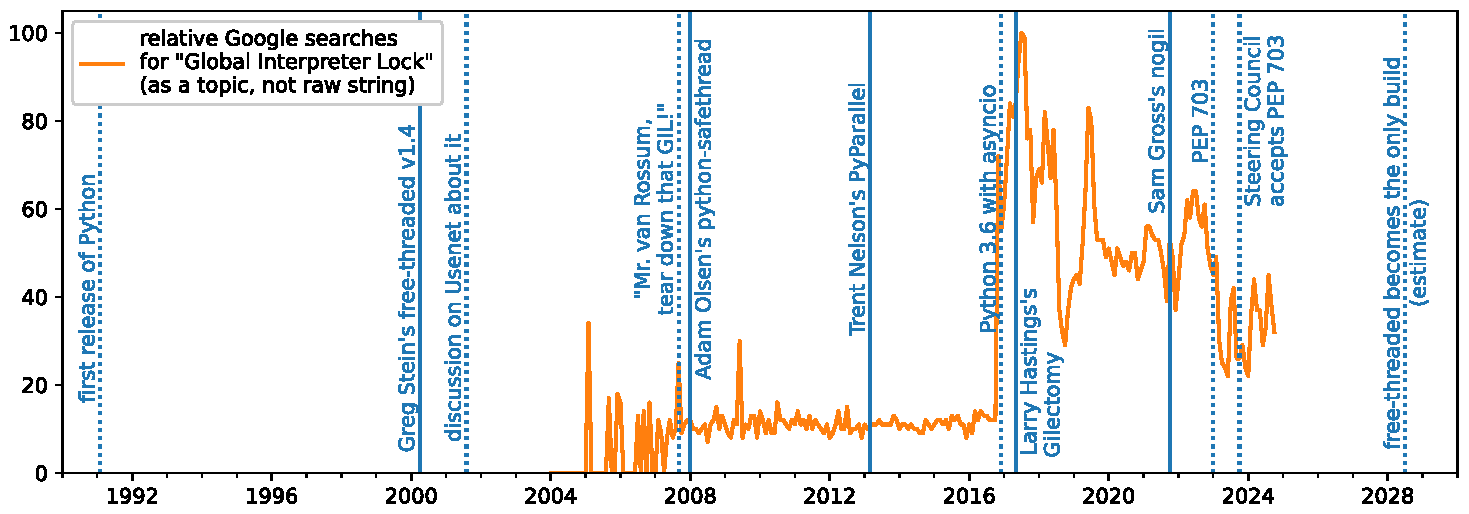
\includegraphics[width=\linewidth]{img/googletrends-gil-timeline.pdf}
\end{columns}

\vspace{0.5 cm}
\uncover<2->{Five forked Pythons, in 2000, 2008, 2013, 2017, 2021, experimentally disabled the GIL.}

\vspace{0.25 cm}
\uncover<3->{Until recently, they all made single (and sometimes multi) threaded performance \underline{\it worse}.}
\end{frame}

\begin{frame}[fragile]{Why is it working now?}
\vspace{0.5 cm}
\large
The main issue was CPython's ubiquitous reference counting. Replacing

\vspace{0.1 cm}
\begin{minted}{c}
    ((PyObject*)(obj))->ob_refcnt++;
\end{minted}

\vspace{0.1 cm}
with an atomic operation (or similar) is expensive because it is called so often.

\vspace{0.5 cm}
\uncover<2->{J.~Choi, T.~Shull, J.~Torrellas, {\it Biased reference counting: minimizing atomic operations in garbage collection}, PACT'18 (\textcolor{blue}{\href{https://doi.org/10.1145/3243176.3243195}{DOI 10.1145/3243176.3243195}}).}

\vspace{0.25 cm}
\uncover<3->{Most objects are only referenced by the thread in which they were created.}

\begin{center}
\uncover<4->{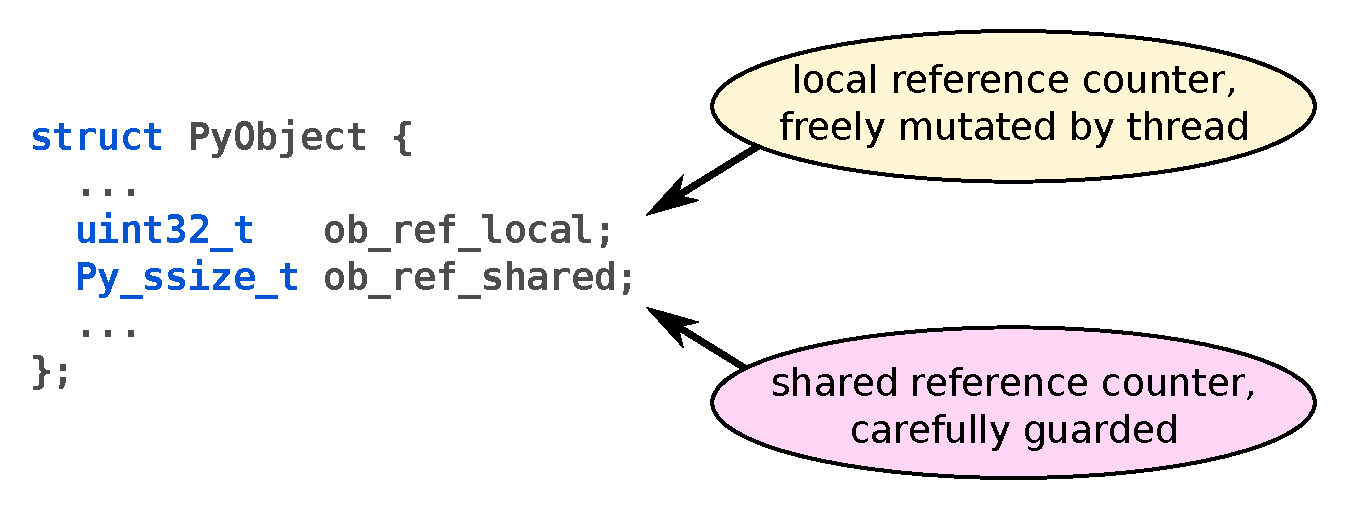
\includegraphics[width=0.63\linewidth]{img/two-reference-counters.pdf}}
\end{center}
\end{frame}

\begin{frame}{Also\ldots \hspace{5 cm} \small\url{https://peps.python.org/pep-0703}}
\vspace{0.5 cm}
\large
\begin{itemize}
\item no reference counting of immortal objects: \mintinline{python}{None}, \mintinline{python}{True}, \mintinline{python}{False}, small integers, interned strings\ldots
\item deferred reference counting: top-level functions, code objects, modules, methods tend to be accessed by many threads; don't reference count, only garbage collect
\item replacing PyMalloc (for small Python objects) with mimalloc
\item no linked lists in garbage collecting
\item no more generational garbage collecting (reference counting handles short-lived objects)
\item locks on all mutable containers (lists, dicts) with optimistic access
\item alternatives to borrowed references in C (\mintinline{c}{PyList_GetItem} $\to$ \mintinline{c}{PyList_FetchItem})
\item ``critical sections'' in bytecode sequences to avoid deadlocks
\end{itemize}
\end{frame}

\begin{frame}
\vspace{1 cm}
\LARGE
\begin{center}
\textcolor{darkblue}{Scaling tests}
\end{center}
\end{frame}

\begin{frame}[fragile]{Something computationally expensive in pure Python}
\vspace{0.4 cm}
\scriptsize
\begin{minted}{python}
# Can't use NumPy in subinterpreters, so use Python's built-in array instead.
offsets = (ctypes.c_int64 * (N + 1)).from_address(ptr_offsets)
pt = (ctypes.c_float * offsets[-1]).from_address(ptr_pt)
eta = (ctypes.c_float * offsets[-1]).from_address(ptr_eta)
phi = (ctypes.c_float * offsets[-1]).from_address(ptr_phi)
mass = (ctypes.c_float * N).from_address(ptr_mass)

# Dimuon mass on all combinations of muons per event...
for event in range(start, stop):
    max_mass = 0
    for i in range(offsets[event], offsets[event + 1]):
        pt1 = pt[i]
        eta1 = eta[i]
        phi1 = phi[i]
        for j in range(i + 1, offsets[event + 1]):
            pt2 = pt[j]
            eta2 = eta[j]
            phi2 = phi[j]
            m = sqrt(2*pt1*pt2*(cosh(eta1 - eta2) - cos(phi1 - phi2)))
            if m > max_mass:
                max_mass = m
    mass[event] = max_mass
\end{minted}
\end{frame}

\begin{frame}{Scaling test results (8 physical cores)}
\large
\vspace{0.5 cm}
\begin{columns}
\column{0.8\linewidth}
\only<1>{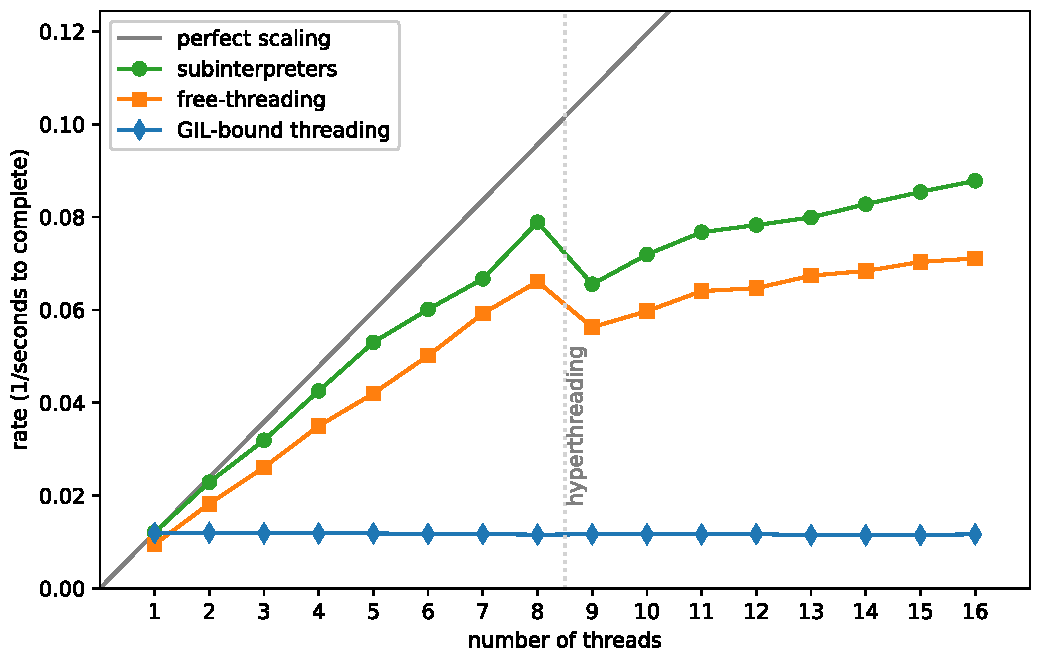
\includegraphics[width=\linewidth]{img/scaling-of-compute-basic.pdf}}\only<2>{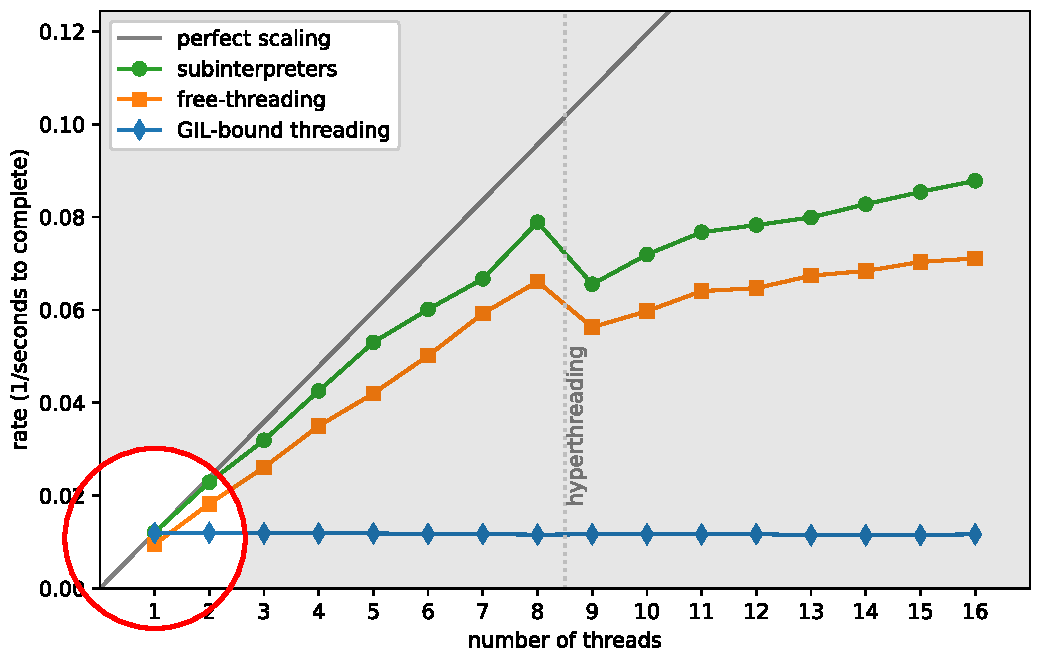
\includegraphics[width=\linewidth]{img/scaling-of-compute-circle.pdf}}\only<3>{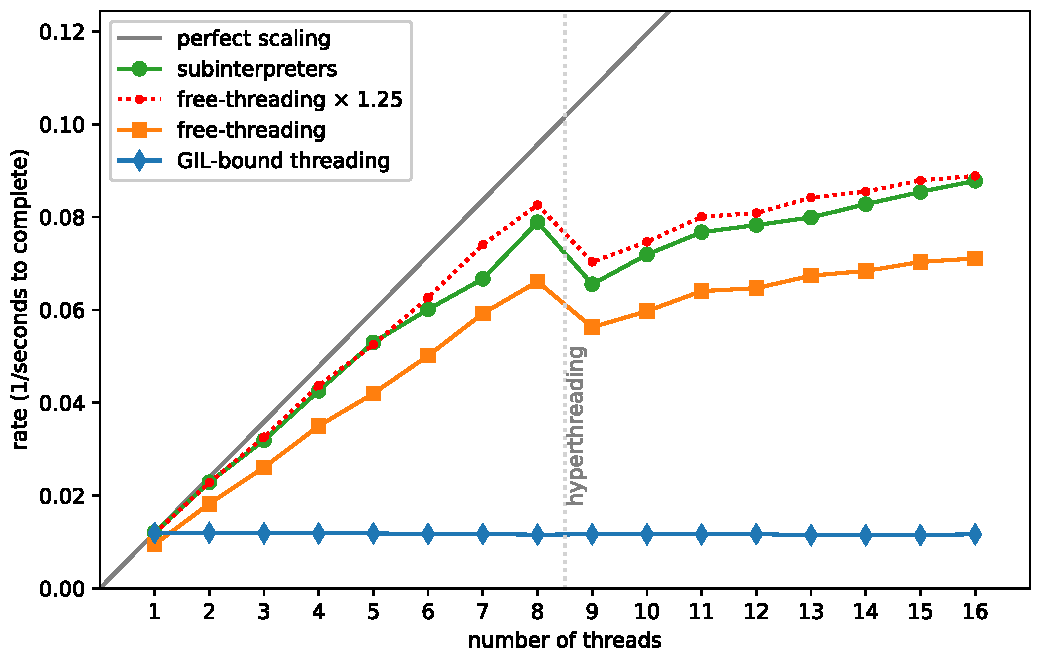
\includegraphics[width=\linewidth]{img/scaling-of-compute-extra.pdf}}

\column{0.25\linewidth}
\only<1>{Subinterpreters and free-threading both escape single-thread scaling limit.}\only<2>{Free-threading doesn't have all the latest optimizations; single-threaded is slower (for now).}\only<3>{In fact, it's a constant factor.}
\end{columns}
\end{frame}

\begin{frame}{CPUs are constantly busy, even though scaling isn't perfect}
\Large
\vspace{0.25 cm}
\begin{center}
\begin{onlyenv}<1>
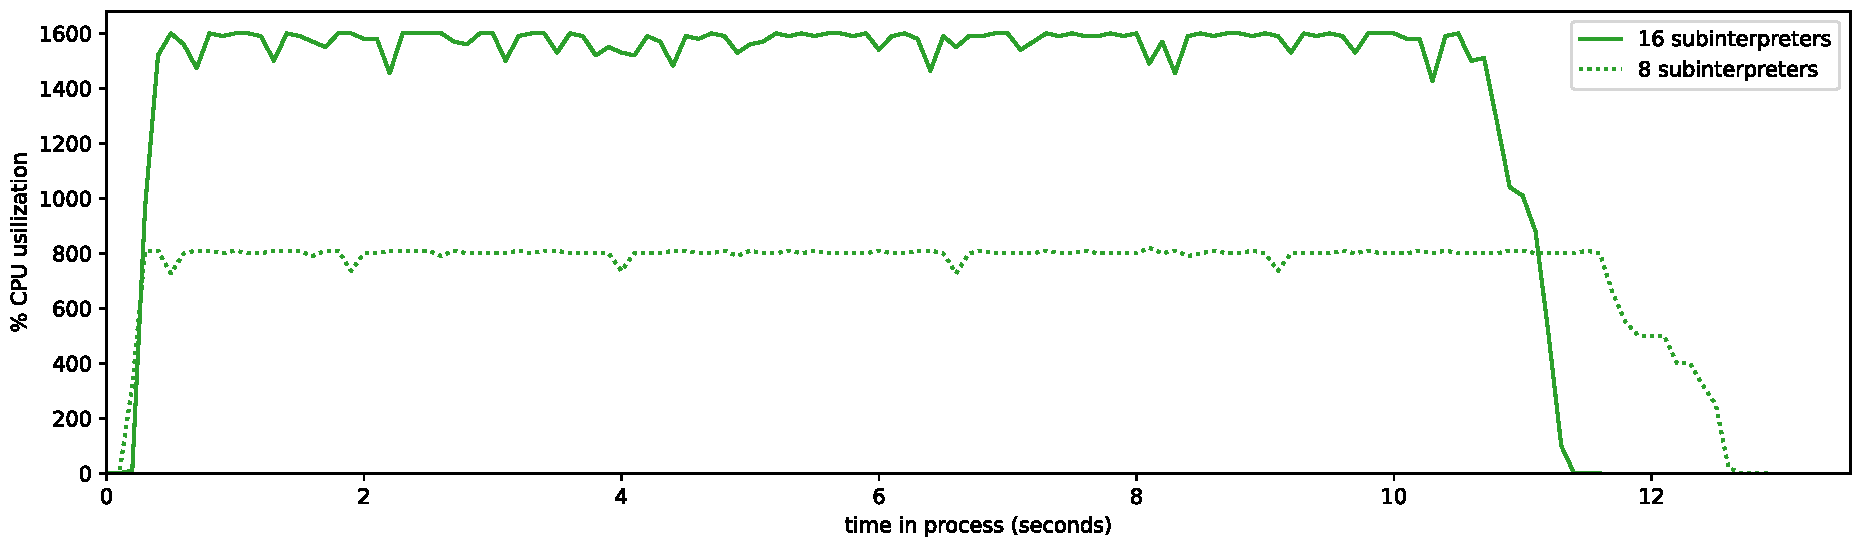
\includegraphics[width=0.93\linewidth]{img/cpu-of-compute-subinterpreters.pdf}

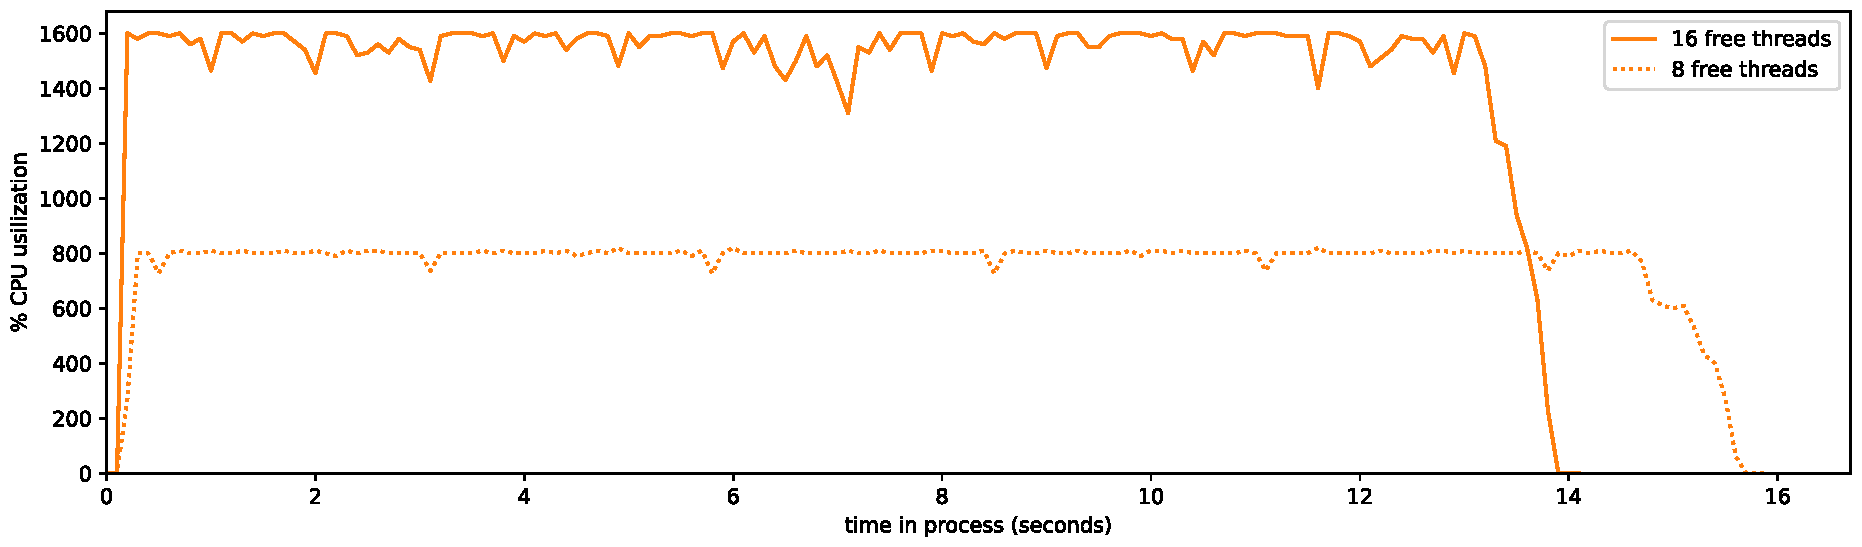
\includegraphics[width=0.93\linewidth]{img/cpu-of-compute-free-threads.pdf}
\end{onlyenv}\begin{onlyenv}<2>
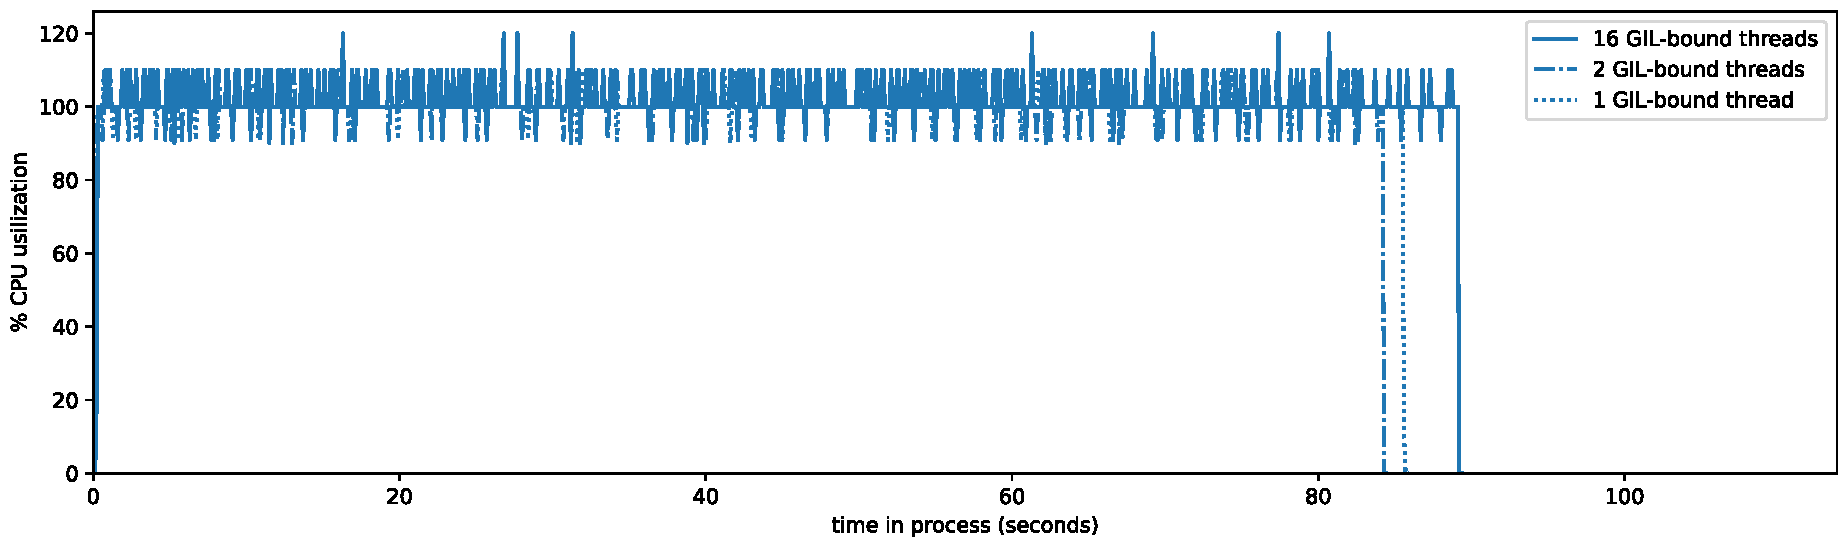
\includegraphics[width=0.93\linewidth]{img/cpu-of-compute-gil-threads.pdf}

For a pure Python, computationally intensive workload like this, \\ the GIL strictly limits available threads to 1.
\end{onlyenv}
\end{center}
\end{frame}

\begin{frame}{Can we go further? (48 physical cores)}
\large
\vspace{0.5 cm}
\begin{columns}
\column{0.8\linewidth}
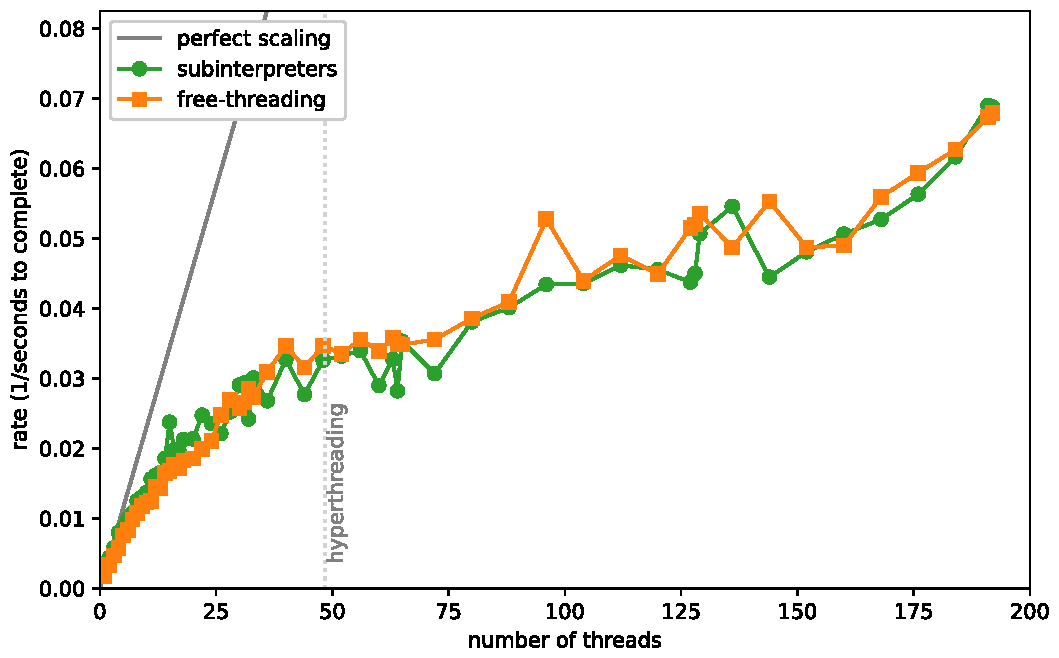
\includegraphics[width=\linewidth]{img/scaling-of-compute-big.pdf}

\column{0.25\linewidth}
The hyperthreading threshold doesn't look significant on this hardware (AWS c7i.metal-48xl).
\end{columns}
\end{frame}

\begin{frame}{Not all threads finish equal work in equal times}
\vspace{0.25 cm}
\begin{center}
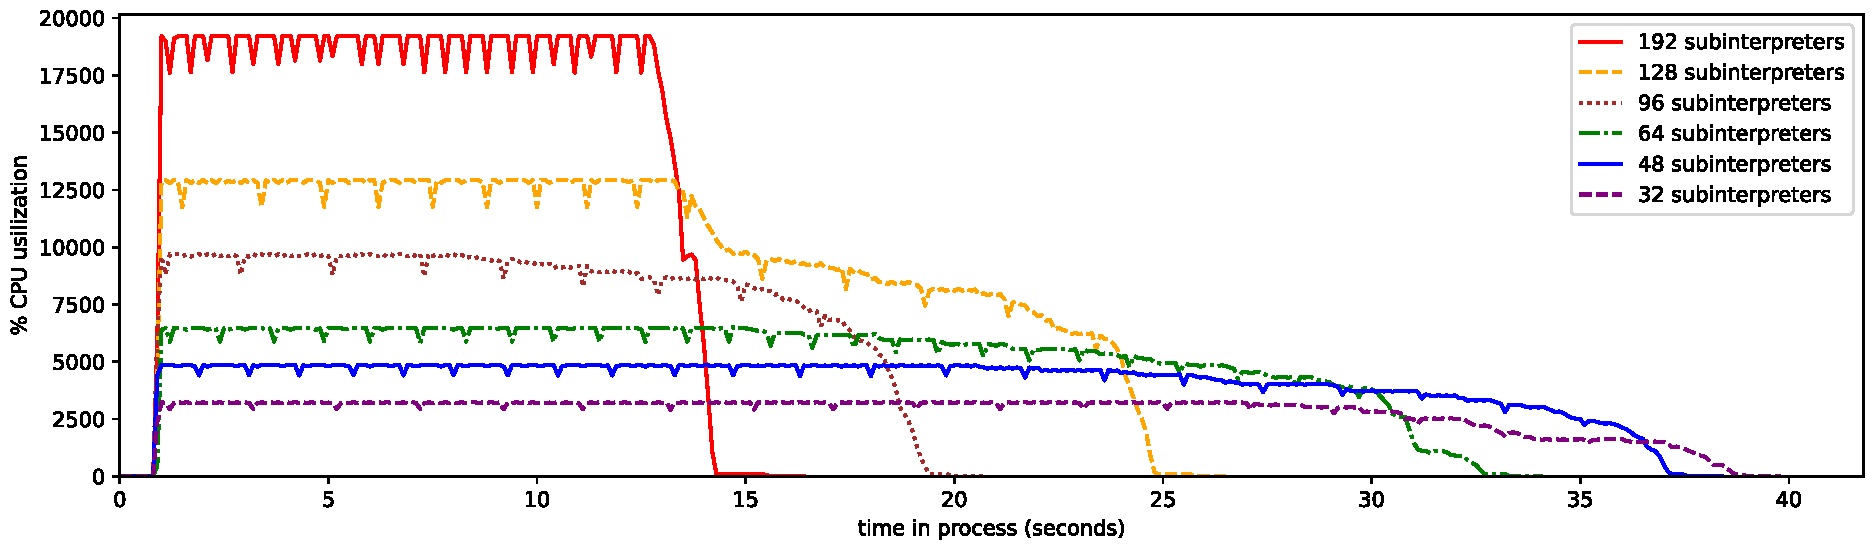
\includegraphics[width=0.93\linewidth]{img/cpu-of-compute-subinterpreters-big.pdf}

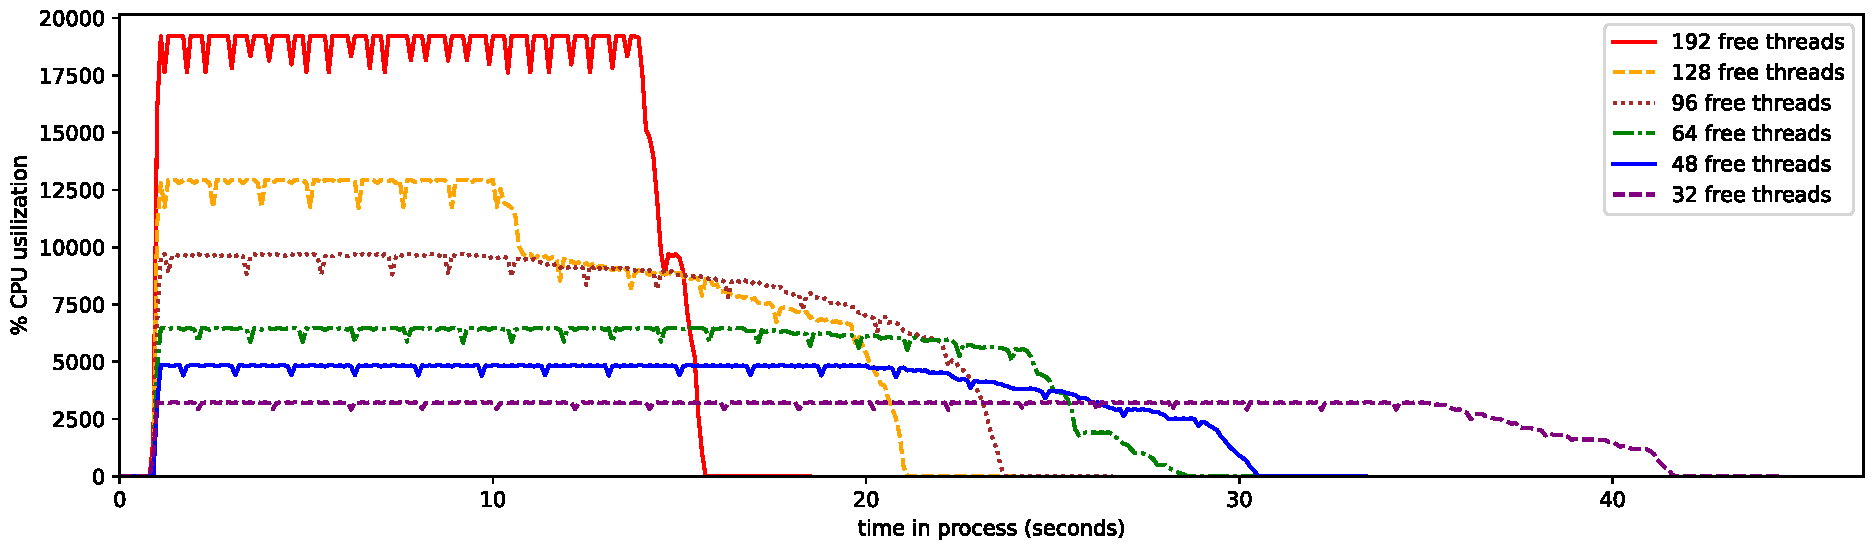
\includegraphics[width=0.93\linewidth]{img/cpu-of-compute-free-threads-big.pdf}
\end{center}
\end{frame}

\begin{frame}
\vspace{1 cm}
\LARGE
\begin{center}
\textcolor{darkblue}{Scaling tests with Uproot}
\end{center}
\end{frame}

\begin{frame}[fragile]{Uproot has already been (partly) evading the GIL}
\large
\vspace{0.7 cm}

Most computationally intensive work is offloaded to NumPy and Awkward Array, which release the GIL before numerical computations.

\small
\vspace{0.1 cm}
\begin{minted}{c}
   Py_BEGIN_ALLOW_THREADS;                // releases the GIL

   big_computation_without_PyObjects();   // other threads run, too

   Py_END_ALLOW_THREADS;                  // re-acquires the GIL

   return result_with_PyObjects;
\end{minted}

\large
\vspace{0.4 cm}
\uncover<2->{But we only enter GIL-released C code on a per-TBasket basis.}

\vspace{0.4 cm}
\uncover<2->{The code between these excursions are synchronization points (Amdahl's law).}
\end{frame}

\begin{frame}[fragile]{Two ways to parallelize Uproot}
\large
\vspace{1 cm}
\hspace{-0.5 cm}\textcolor{darkblue}{``External'':} some code that controls threading (e.g.\ Dask) calls Uproot

\small
\vspace{0.1 cm}
\begin{minted}{python}
def in_thread(uproot_tree, start, stop):
    return uproot_tree.arrays(entry_start=start, entry_stop=stop)

executor = ThreadPoolExecutor(max_workers=N)
batches = executor.map(in_thread, list_of_args_tuples)
\end{minted}

\large
\vspace{0.5 cm}

\hspace{-0.5 cm}\textcolor{darkblue}{``Internal'':} Uproot reads TBaskets in parallel but returns one array

\small
\vspace{0.1 cm}
\begin{minted}{python}
executor = ThreadPoolExecutor(max_workers=N)

array = uproot_tree.arrays(
    decompression_executor=executor, interpretation_executor=executor
)
\end{minted}
\end{frame}

\begin{frame}{Parallelizing Uproot ``externally''}
\large
\vspace{0.5 cm}
\begin{columns}
\column{0.8\linewidth}
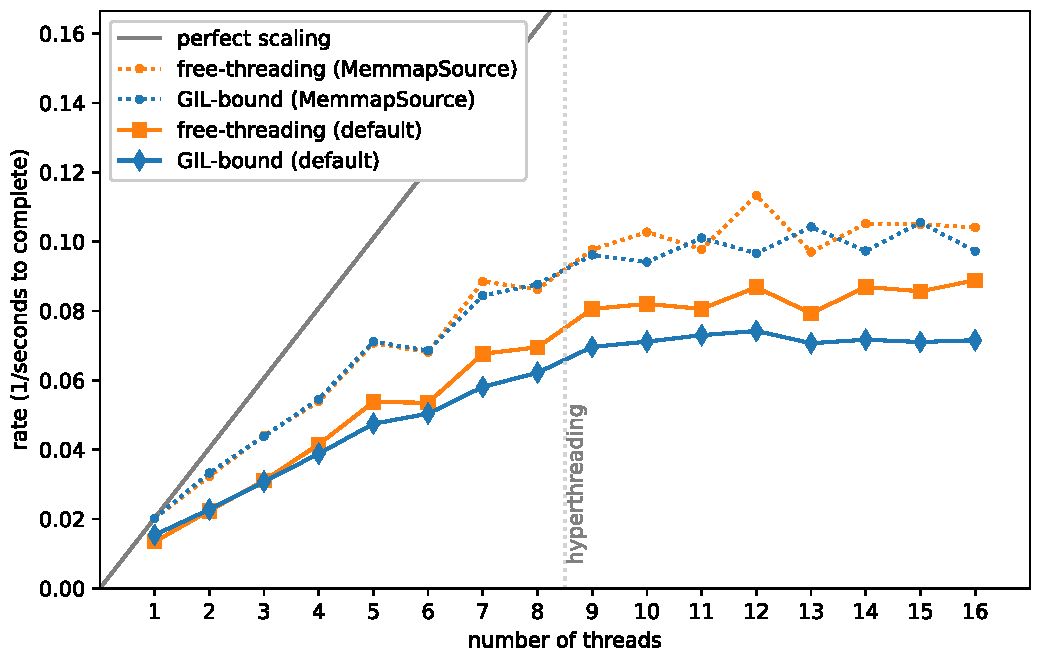
\includegraphics[width=\linewidth]{img/scaling-of-uproot-external.pdf}

\column{0.25\linewidth}
GIL-bound is not bad, but there's a small improvement.

\vspace{0.5 cm}
The bigger difference is between the default file \mintinline{python}{handler} and \mintinline{python}{MemmapSource}.

\vspace{\baselineskip}
\end{columns}
\end{frame}

\begin{frame}{Parallelizing Uproot ``internally''}
\large
\vspace{0.5 cm}
\begin{columns}
\column{0.8\linewidth}
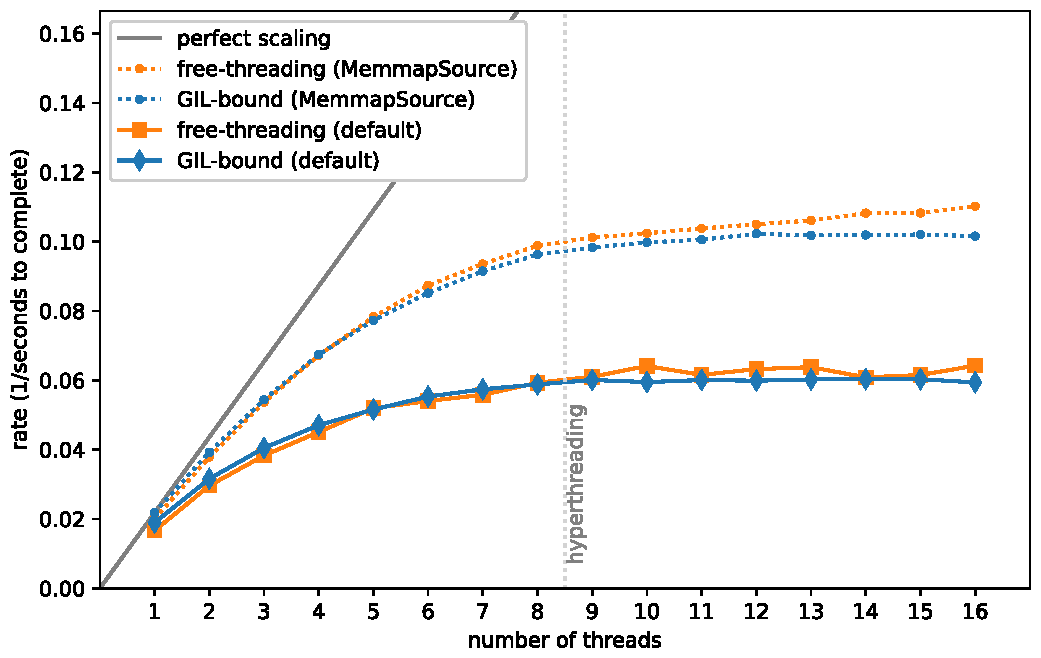
\includegraphics[width=\linewidth]{img/scaling-of-uproot-internal.pdf}

\column{0.25\linewidth}
GIL-bound is not bad, but there's a small improvement.

\vspace{0.5 cm}
Especially in the internal case \textcolor{gray}{(more fine-grained; less waste from multiple threads reading the same TBaskets)}.
\end{columns}
\end{frame}

\begin{frame}{CPUs are not always busy, but free-threaded is busier\ldots}
\vspace{1 cm}
\begin{center}
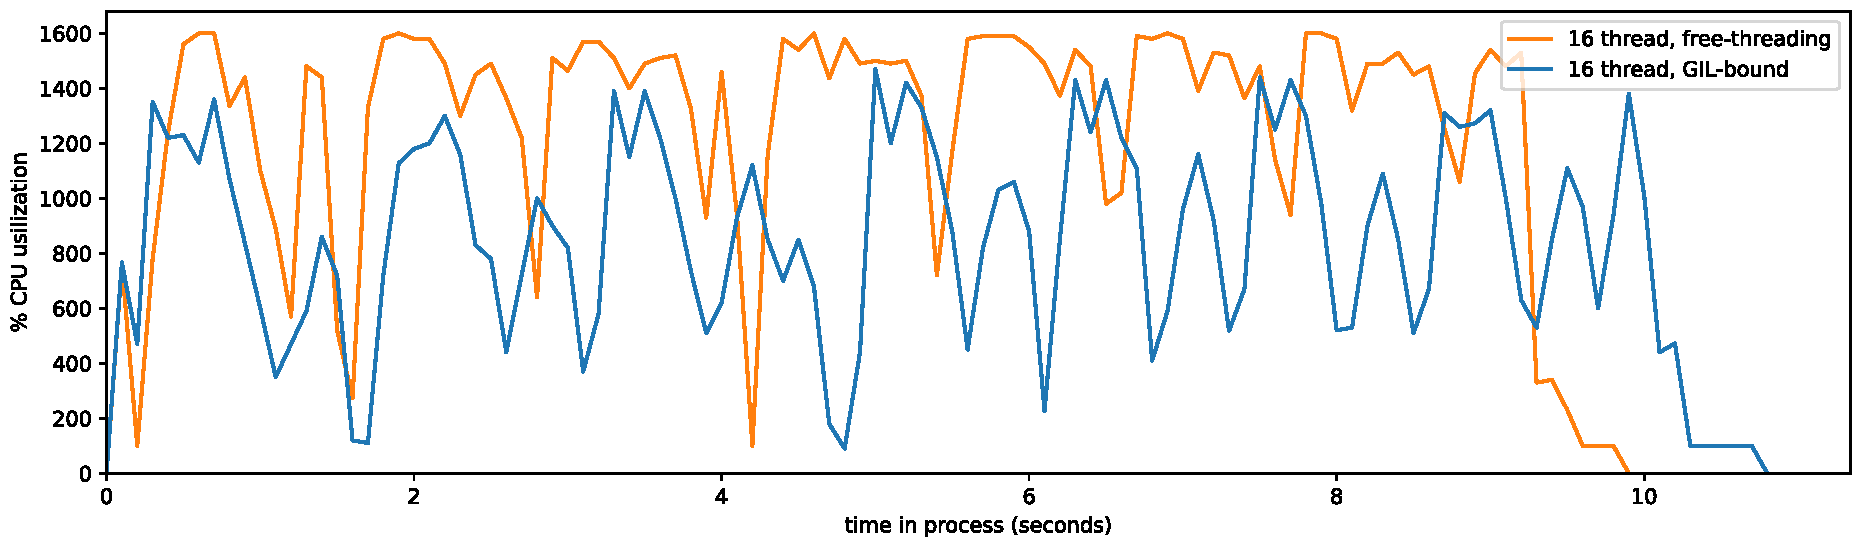
\includegraphics[width=0.93\linewidth]{img/cpu-of-uproot-internal-16.pdf}

\vspace{0.5 cm}
Note: file-reading tasks performed with warm cache, so RAM $\to$ CPU is the only I/O.
\end{center}
\end{frame}

\begin{frame}{Can we go further? (48 physical cores, ``internal'' parallelization)}
\large
\vspace{0.5 cm}
\begin{columns}
\column{0.8\linewidth}
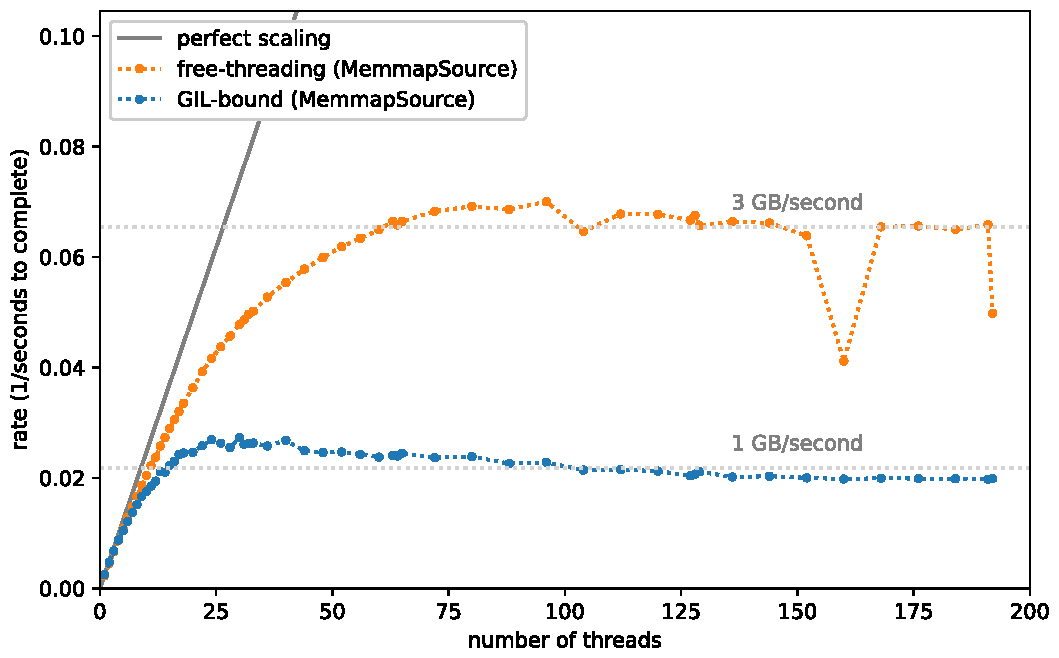
\includegraphics[width=\linewidth]{img/scaling-of-uproot-internal-big.pdf}

\column{0.25\linewidth}
Free-threading starts to be relevant above 8 threads and keeps getting better until 3~GB/second.

\vspace{1 cm}
You need well over 8 cores to see this.
\end{columns}
\end{frame}

\begin{frame}{CPUs are still not always busy, but free-threaded is busier\ldots}
\vspace{0.25 cm}
\begin{center}
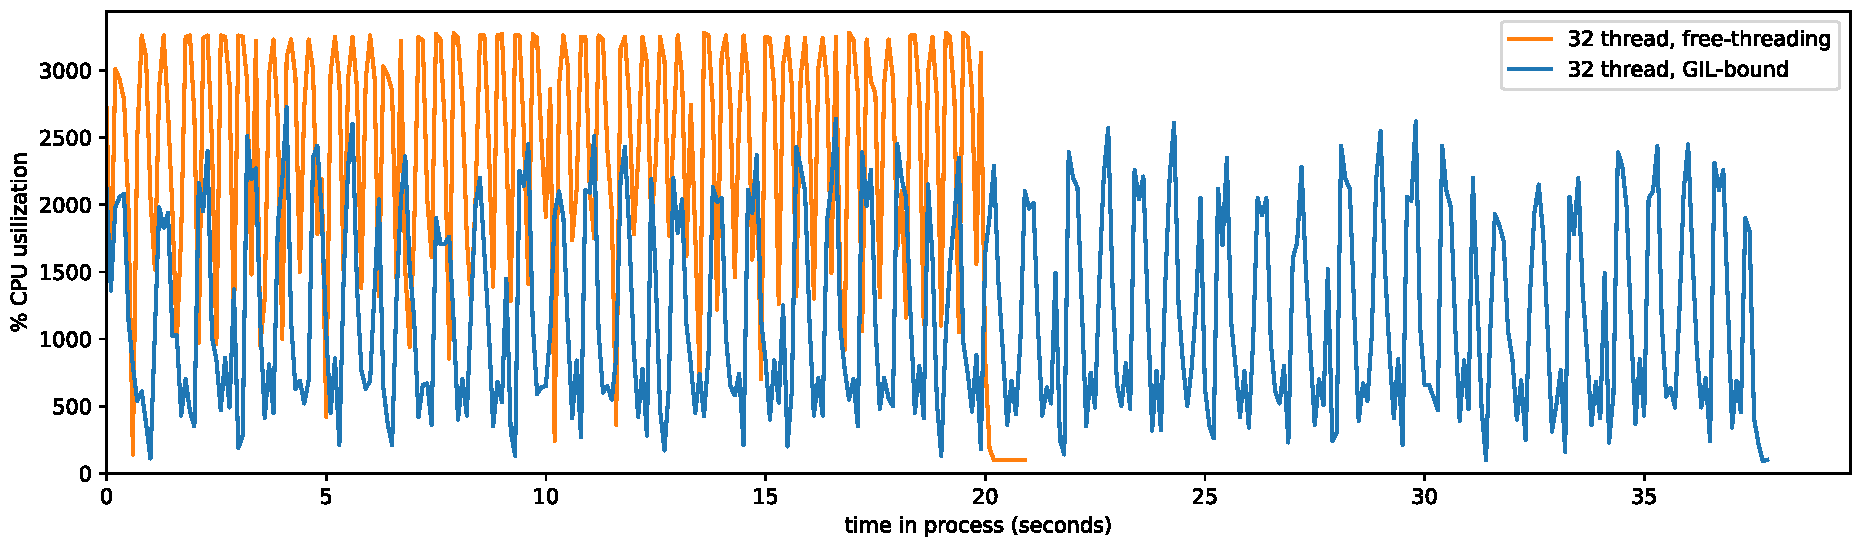
\includegraphics[width=0.93\linewidth]{img/cpu-of-uproot-internal-big-32.pdf}

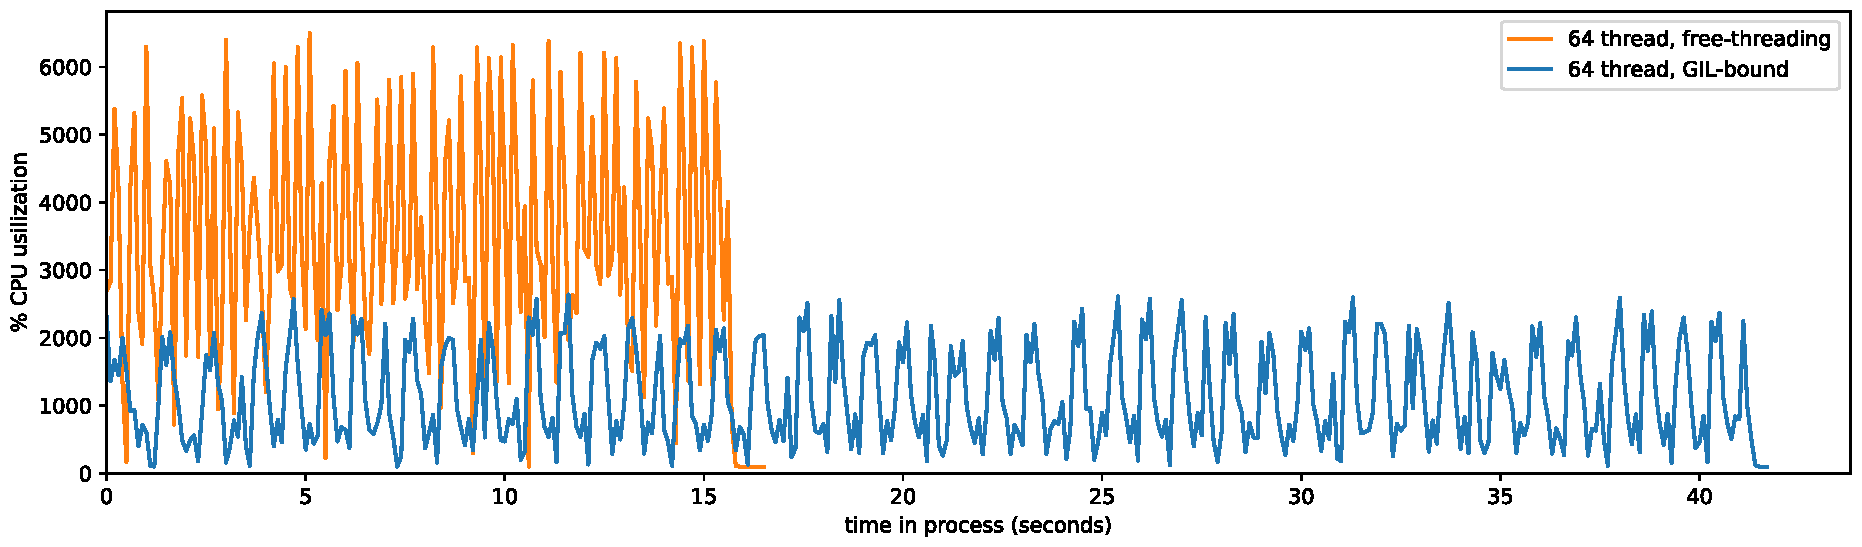
\includegraphics[width=0.93\linewidth]{img/cpu-of-uproot-internal-big-64.pdf}
\end{center}
\end{frame}

\begin{frame}{Conclusions}
\vspace{0.3 cm}
\Large
\begin{itemize}\setlength{\itemsep}{0.2 cm}
\item<1-> Python 3.13 provides two new ways to avoid the GIL.
\item<2-> {\bf Subprocessors} require more effort from Python users and are not well supported by libraries (NumPy).
\item<3-> {\bf Free-threading} required a massive overhaul of Python's internals, but ``just works'' from a Python user's perspective.

\vspace{0.2 cm}
\uncover<4->{\textcolor{gray}{(Python community is much more interested in free-threading.)}}

\vspace{0.1 cm}
\item<5-> They scale identically, apart from a constant factor (bytecode optimizations, to be implemented later in free-threading mode).
\item<6-> Uproot has already been releasing the GIL, but benefits from free-threading if you have a lot more than 8 cores.
\end{itemize}
\end{frame}

\end{document}
